\chapter{Analysis}

% TODO: Cite?
Once we had a working Android application, we performed experiments on a Motorola Moto G5s Plus phone with Android version Nougat 7.1. We also used an external speaker to create acoustic signals at loud volume (\~70dB).

We use Python and it's scientific suite (Numpy, Scipy, Pandas etc.) to perform analysis and create plots.

Our android application stores the audio files in M4A format because that is what the Android APIs allow, but to make processing easier we use the FFmpeg tool to convert these M4As to WAV files as there are a lot more libraries that support WAV out of the box.

The experimentation was straightforward - try playing loud audio signal in the vicinity of the phoen, and see if the accelerometer data shows a response.

According to the Nyquist sampling theorem a sampling frequency f enables us to reconstruct signals at frequencies of up to f/2. Since the frequency of an Android motion sensor is limited to be 200Hz, this allows us to directly sense audio signals of up to 100 Hz.

But, there is also a separate effect of Aliasing \cite{gyrophone} - a phenomenon where for a sinusoid of frequency F, sampled with frequency f, the resulting samples are indistinguishable from those of another sinusoid of frequency | F − n*f |, for any integer N. The values corresponding to N != 0 are called images or aliases of frequency f. An undesirable phenomenon in general, here aliasing allows us to sense audio signals having frequencies which are higher than 100 Hz, thereby extracting more information from the gyroscope readings.

So, if we play a tone of 270Hz near an accelerometer (or a gyroscope for that matter) we expect to see peaks in the Fast Fourier Transform curve of the signal at around 70Hz.

The results of this experiment are shown in the figures that follow. The first graph is the signal itself, the second is the FFT curve of the signals, showing the dominant frequencies and the third is the spectrogram, showing when the frequencies are high (darker color in the spectrogram).

% Playing tones of various frequencies
% In different positions of the phone (since motion sensors have axes)
% Plotted waveform, fft, spectrogram of microphone, gyroscope, \& accelerometer.

% Signal analysis shows positive results
% Both Gyroscope \& Accelerometer are affected by acoustic signals

\begin{figure}[H] \begin{center}
\makebox[\textwidth][c]{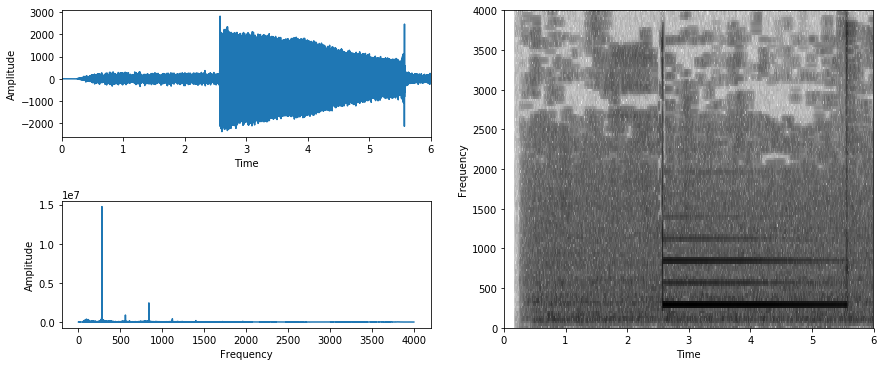
\includegraphics[width=1.3\textwidth]{analysis_mic}}
\caption{Microphone (when playing a 270 Hz audio wave)}
\label{fig:analysis_mic}
\end{center} \end{figure}

\begin{figure}[H] \begin{center}
\makebox[\textwidth][c]{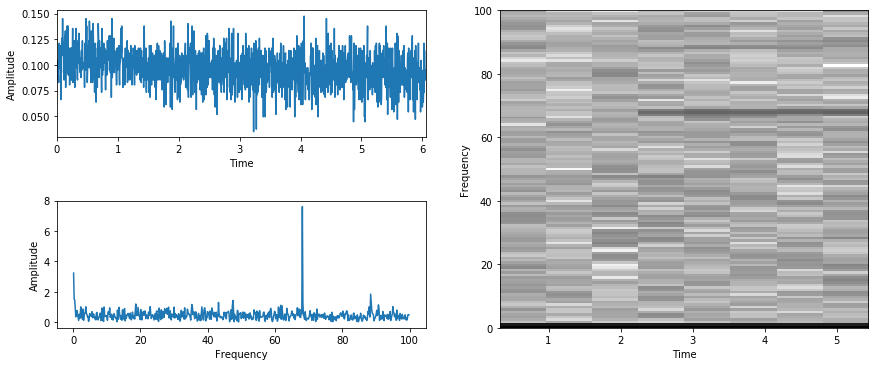
\includegraphics[width=1.3\textwidth]{analysis_acc}}
\caption{Accelerometer (when playing a 270 Hz audio wave)}
\label{fig:analysis_acc}
\end{center} \end{figure}

\begin{figure}[H] \begin{center}
\makebox[\textwidth][c]{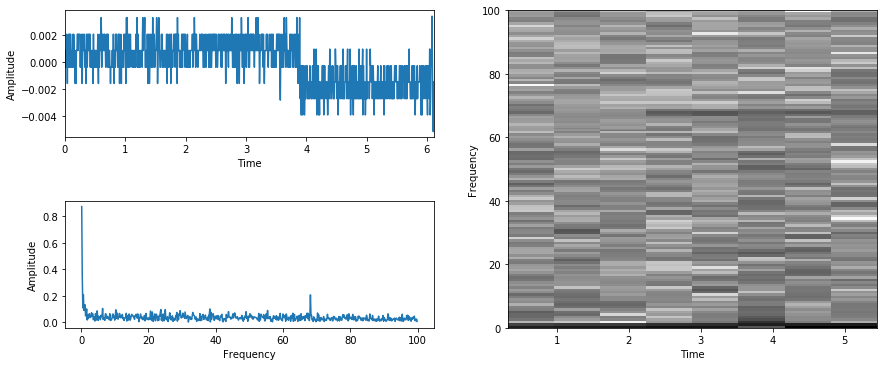
\includegraphics[width=1.3\textwidth]{analysis_gyr}}
\caption{Gyroscope (when playing a 270 Hz audio wave)}
\label{fig:analysis_gyr}
\end{center} \end{figure}

As can be seen from figure \ref{fig:analysis_mic}, the 270Hz tone begins at around 2.5 seconds, and its FFT clearly shows a distinct peak at 270Hz. The spectrogram is dense since there's a lot of data (as microphones sample at rates close to 8000Hz) but we can clearly observe that from 2.5 seconds to 5.5 seconds, there are multiple frequency bands (which are just aliases of each other.)

What is more interesting is figure \ref{fig:analysis_acc} where just from looking at the signal plot, it is not quite evident that there is any particular pattern to it, but the FFT plot again reveals a peak at around 70Hz (this is the aliased frequency of 270Hz.) Looking at the spectrogram we again find that there is a single distinct line at around 70 Hz.

Similar results can be seen in figure \ref{fig:analysis_gyr} but the values are fainter than the accelerometer.

